\section{Introduction}

\begin{frame}{Recap: Self-Attention Mechanism}
    \begin{columns}
        \begin{column}{0.5\textwidth}
            \begin{figure}
                \centering
                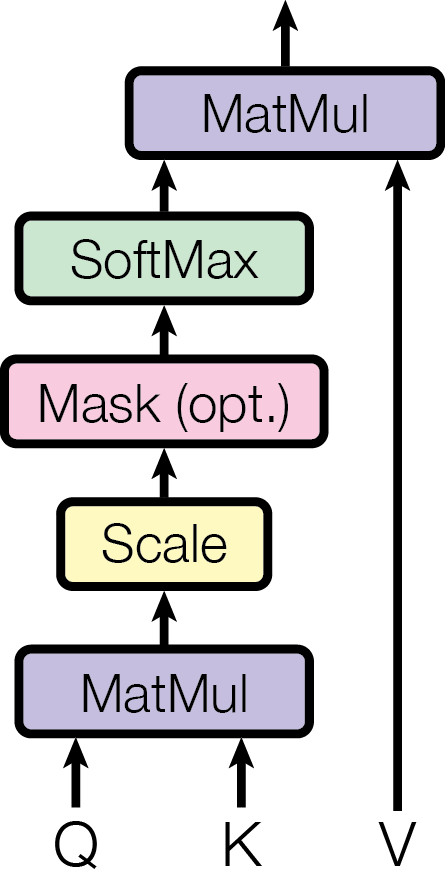
\includegraphics[height=0.75\textwidth]{pic/ModalNet-19}
                \caption{
                Scaled Dot-Product Attention.
                }
                \label{fig:doprod}
            \end{figure}
        \end{column}
        \begin{column}{0.5\textwidth}
            \begin{figure}
                \centering
                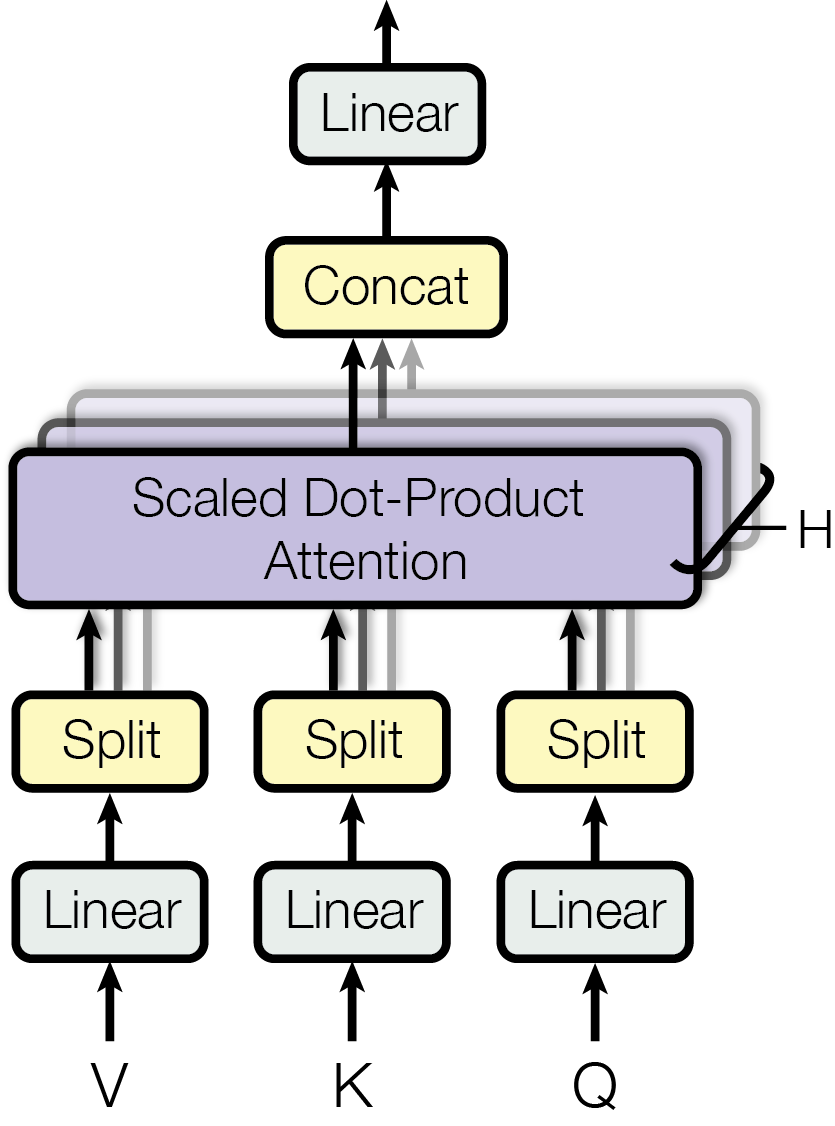
\includegraphics[height=0.75\textwidth]{pic/ModalNet-32}
                \caption{
                Multi-Head Attention consists of several attention layers running in parallel.
                }
                \label{fig:multihead}
            \end{figure}
        \end{column}
    \end{columns}
\end{frame}

% \begin{frame}{Recap: Transformer Architecture}
%     \begin{columns}
%         \begin{column}{0.5\textwidth}
%             \begin{itemize}
%                 \item Transformers have become the model of choice in NLP.
%                 \item The dominant approach is to pre-train on a large text corpus and then fine-tune on a smaller task-specific dataset.
%                 \item Transformers have revolutionized NLP.
%             \end{itemize}
%         \end{column}
%         \begin{column}{0.5\textwidth}
%             \begin{figure}
%                 \centering
%                 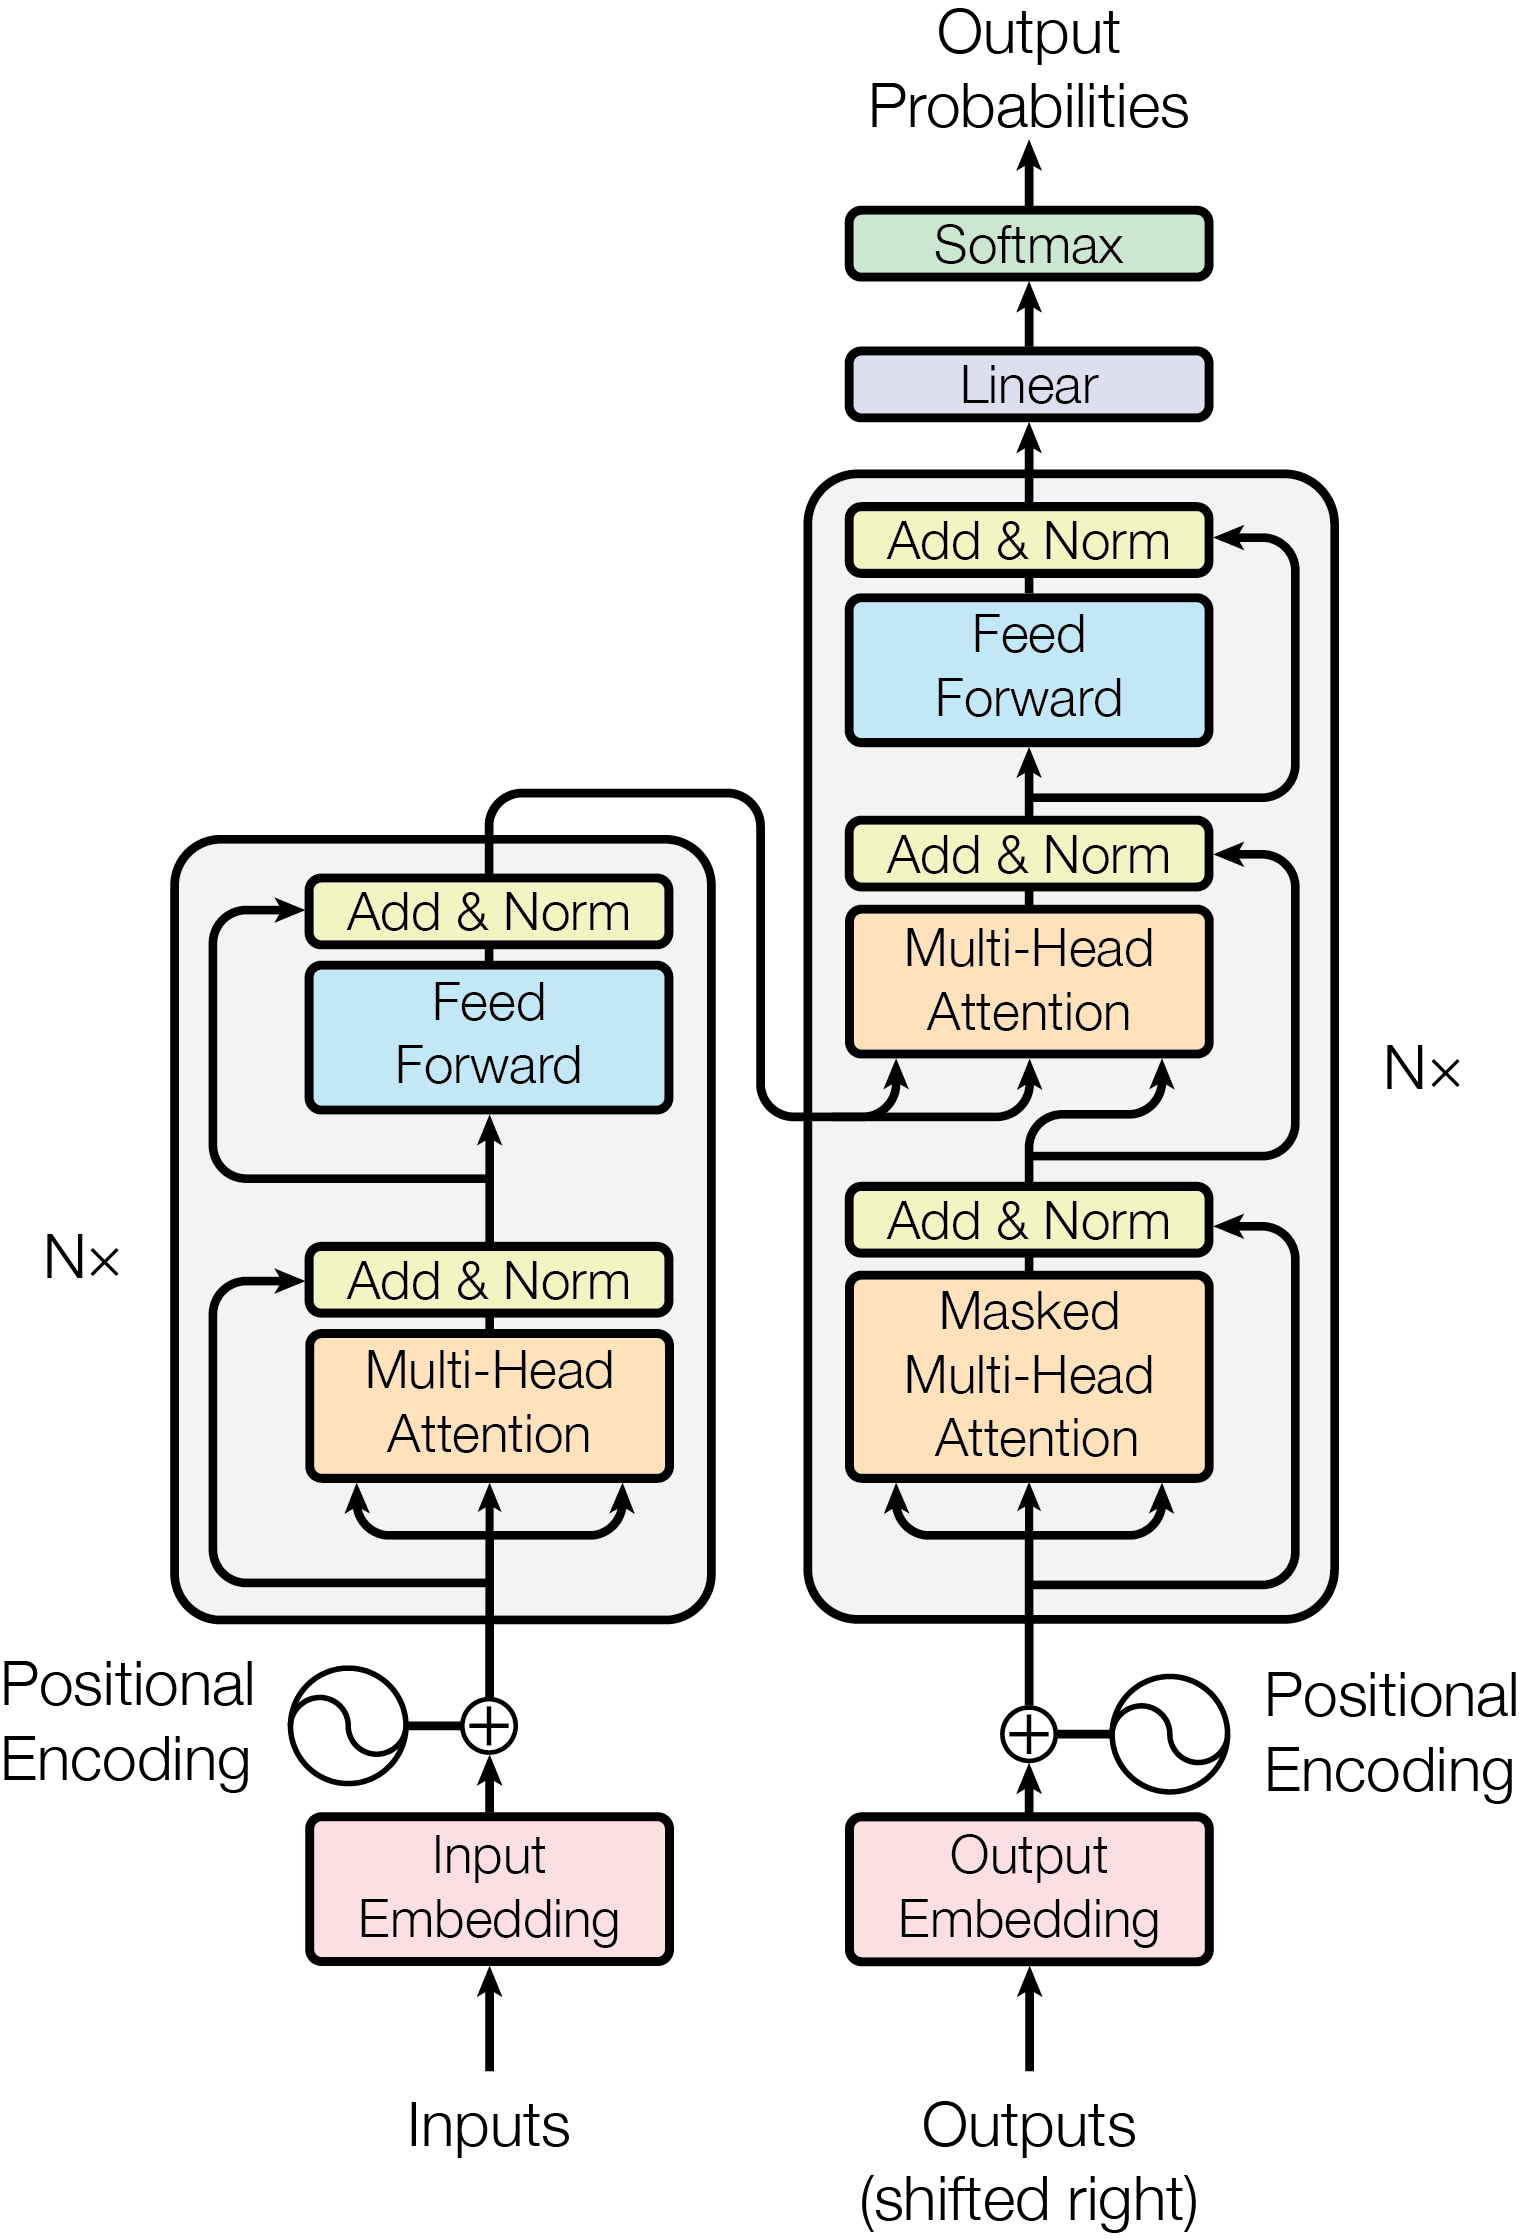
\includegraphics[height=\textwidth]{pic/ModalNet-21}
%                 \label{fig:transformer}
%             \end{figure}
%         \end{column}
%     \end{columns}
% \end{frame}


\begin{frame}{Strengths and Limitations of CNNs}
    \begin{columns}
        \begin{column}{0.55\linewidth}
            \begin{itemize}
                \item CNNs excel at:
                \begin{itemize}
                    \item \emph{Local Feature Extraction} 
                    \item \emph{Translation Invariance} 
                    \item \emph{Efficient Computation} 
                \end{itemize}
                \item However, they have limitations due to:
                \begin{itemize}
                    \item \emph{Limited Receptive Field} 
                    \item \emph{Pooling Information Loss} 
                    \item \emph{Struggle with Global Context} 
                \end{itemize}
            \end{itemize}
        \end{column}
        \begin{column}{0.45\linewidth}
            \begin{figure}
                \centering
                \includesvg[width=\linewidth]{pic/ResNet_block}
                \caption{Block diagram of ResNet}
                \label{fig:resnet}
            \end{figure}
        \end{column}
    \end{columns}
\end{frame}




% \begin{frame}{CNNs Struggle with Global Context}
%     \begin{itemize}
%         \item Why it matters: For tasks that require understanding the entire image (e.g., image classification, where the relationship between distant parts of the image may be important), CNNs often require deep architectures to get the full picture.
%         \item Feature Hierarchy: CNNs build a hierarchical structure of features but rely on many layers to achieve global understanding, leading to more complexity.
%     \end{itemize}
% \end{frame}

